% Aporte de Darwin Joel Sánchez Vera.
% Las tablas y los gráficos los genera analysis/estadisticas.py.
\subsection{Latencia y rendimiento}
\label{sec:resultados}

Las tablas~\ref{tab:latencias} y~\ref{tab:rendimiento} resumen las 40 corridas medidas de la sesión oficial. Cada fila de latencia reúne 500 RTT y cada valor de rendimiento es la media de cinco corridas. La tabla~\ref{tab:comparacion} expresa cada medida de gRPC como diferencia porcentual respecto a TCP; un valor positivo indica que gRPC obtuvo un valor mayor.

% Generado por analysis/estadisticas.py; no editar a mano.
\begin{table}[htbp]
\centering
\small
\caption{Latencia de ida y vuelta por mecanismo, carga y modo}
\label{tab:latencias}
\begin{tabular}{lllrrrr}
\hline
Mecanismo & Carga & Modo & Media (ms) & Mediana (ms) & Desv. est. (ms) & P95 (ms) \\
\hline
TCP & 100 B & secuencial & 0,1152 & 0,0953 & 0,0579 & 0,1915 \\
TCP & 100 B & concurrente & 0,3110 & 0,3014 & 0,0825 & 0,4472 \\
TCP & 10 KiB & secuencial & 0,2122 & 0,1869 & 0,0740 & 0,3451 \\
TCP & 10 KiB & concurrente & 0,5722 & 0,5455 & 0,1624 & 0,8504 \\
gRPC & 100 B & secuencial & 0,6549 & 0,6171 & 0,2141 & 1,0869 \\
gRPC & 100 B & concurrente & 0,5554 & 0,5166 & 0,1612 & 0,8249 \\
gRPC & 10 KiB & secuencial & 0,7948 & 0,6054 & 0,4450 & 1,7950 \\
gRPC & 10 KiB & concurrente & 0,9080 & 0,6980 & 0,7440 & 2,0868 \\
\hline
\end{tabular}
\end{table}

% Generado por analysis/estadisticas.py; no editar a mano.
\begin{table}[htbp]
\centering
\small
\caption{Rendimiento por mecanismo, carga y modo}
\label{tab:rendimiento}
\begin{tabular}{lllrrr}
\hline
Mecanismo & Carga & Modo & Corridas & Mensajes/s & IC 95 \% ($\pm$) \\
\hline
TCP & 100 B & secuencial & 5 & 7\,960,1 & 1\,082,8 \\
TCP & 100 B & concurrente & 5 & 5\,809,4 & 728,0 \\
TCP & 10 KiB & secuencial & 5 & 4\,533,3 & 989,0 \\
TCP & 10 KiB & concurrente & 5 & 3\,549,3 & 515,4 \\
gRPC & 100 B & secuencial & 5 & 825,6 & 212,0 \\
gRPC & 100 B & concurrente & 5 & 2\,112,9 & 427,3 \\
gRPC & 10 KiB & secuencial & 5 & 773,4 & 367,3 \\
gRPC & 10 KiB & concurrente & 5 & 1\,565,0 & 772,0 \\
\hline
\end{tabular}
\end{table}

% Generado por analysis/estadisticas.py; no editar a mano.
\begin{table}[htbp]
\centering
\small
\caption{RTT medio y diferencia de gRPC respecto a TCP, (gRPC $-$ TCP) / TCP}
\label{tab:comparacion}
\begin{tabular}{llrrrrrr}
\hline
Carga & Modo & TCP (ms) & gRPC (ms) & Media & Mediana & P95 & Rendimiento \\
\hline
100 B & secuencial & 0,1152 & 0,6549 & +468,7 \% & +547,6 \% & +467,5 \% & $-$89,6 \% \\
100 B & concurrente & 0,3110 & 0,5554 & +78,6 \% & +71,4 \% & +84,5 \% & $-$63,6 \% \\
10 KiB & secuencial & 0,2122 & 0,7948 & +274,5 \% & +224,0 \% & +420,1 \% & $-$82,9 \% \\
10 KiB & concurrente & 0,5722 & 0,9080 & +58,7 \% & +27,9 \% & +145,4 \% & $-$55,9 \% \\
\hline
\end{tabular}
\end{table}


La figura~\ref{fig:cajas} muestra la distribución de todos los RTT. Usamos escala logarítmica porque los valores van de 0,08~ms a 6,7~ms y, en escala lineal, las cajas de TCP quedarían aplastadas. La figura~\ref{fig:barras} presenta la media de las corridas con su intervalo de confianza del 95~\%.

\begin{figure}[htbp]
\centering
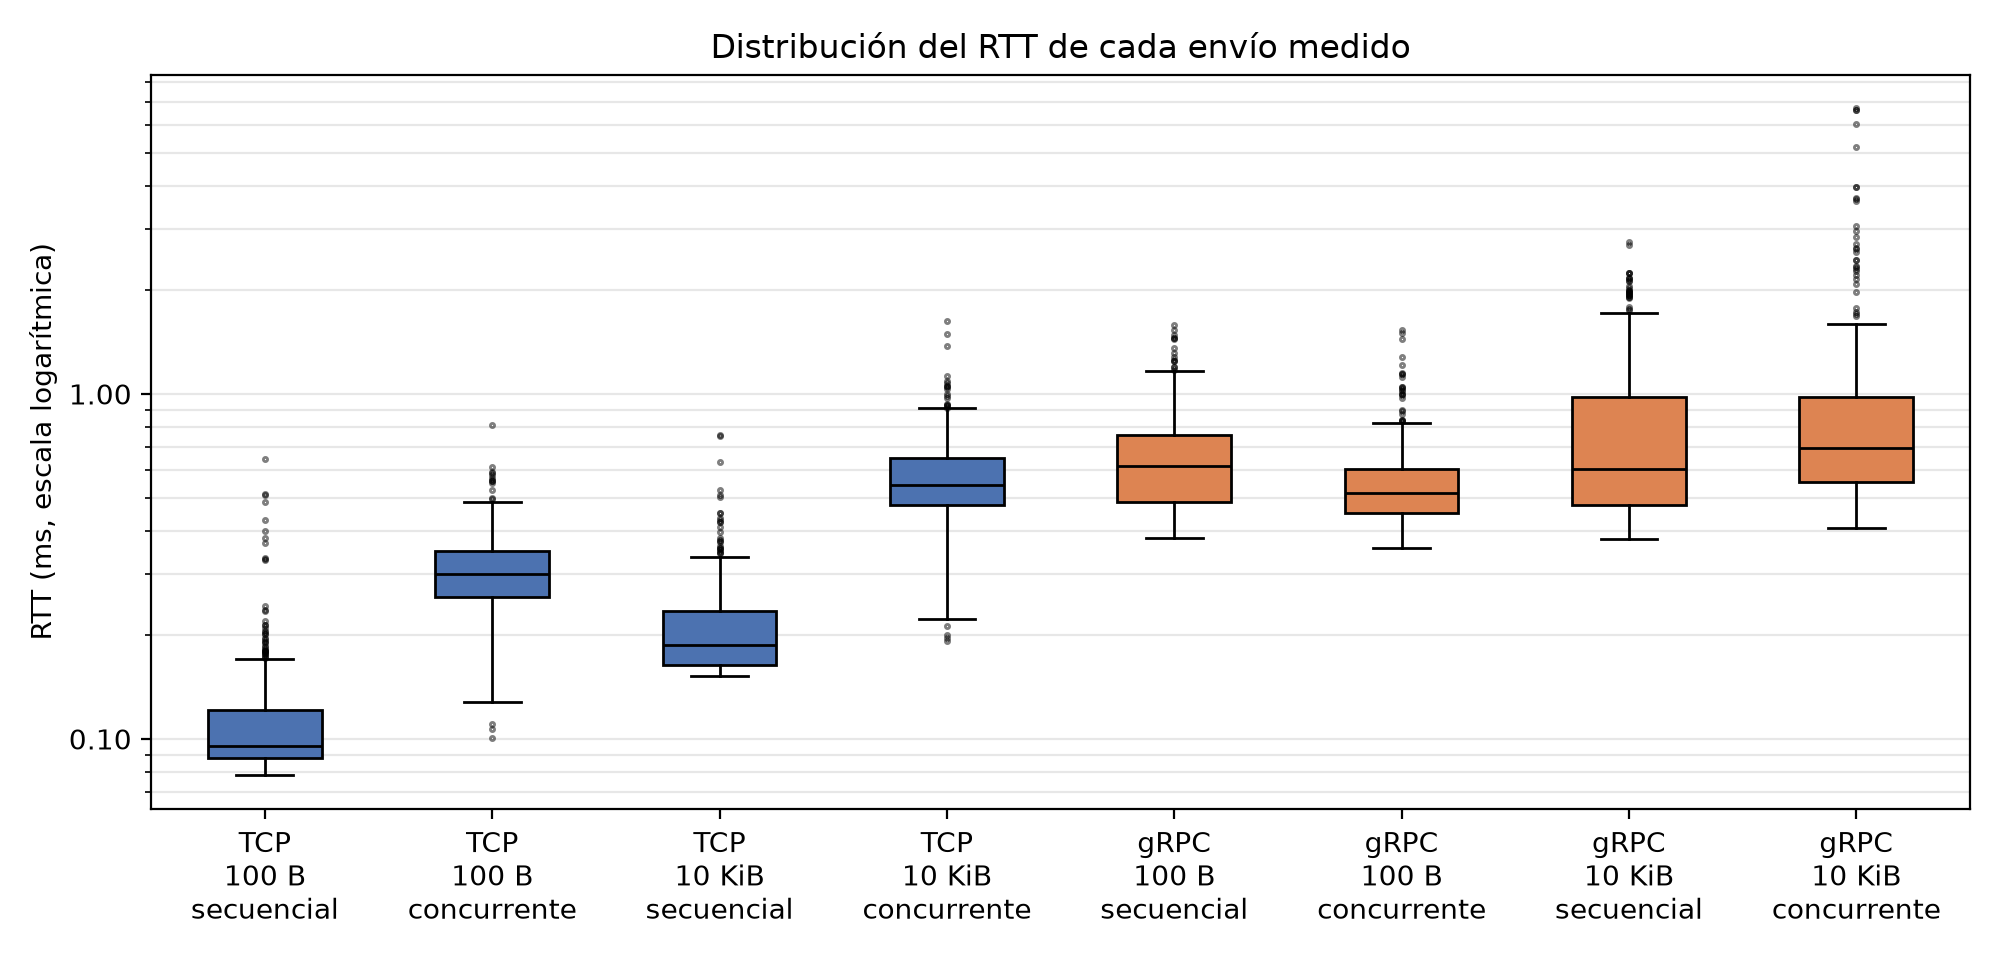
\includegraphics[width=\textwidth]{../analysis/resultados/grafico_cajas.png}
\caption{Distribución del RTT por mecanismo, carga y modo}
\label{fig:cajas}
\end{figure}

\begin{figure}[htbp]
\centering
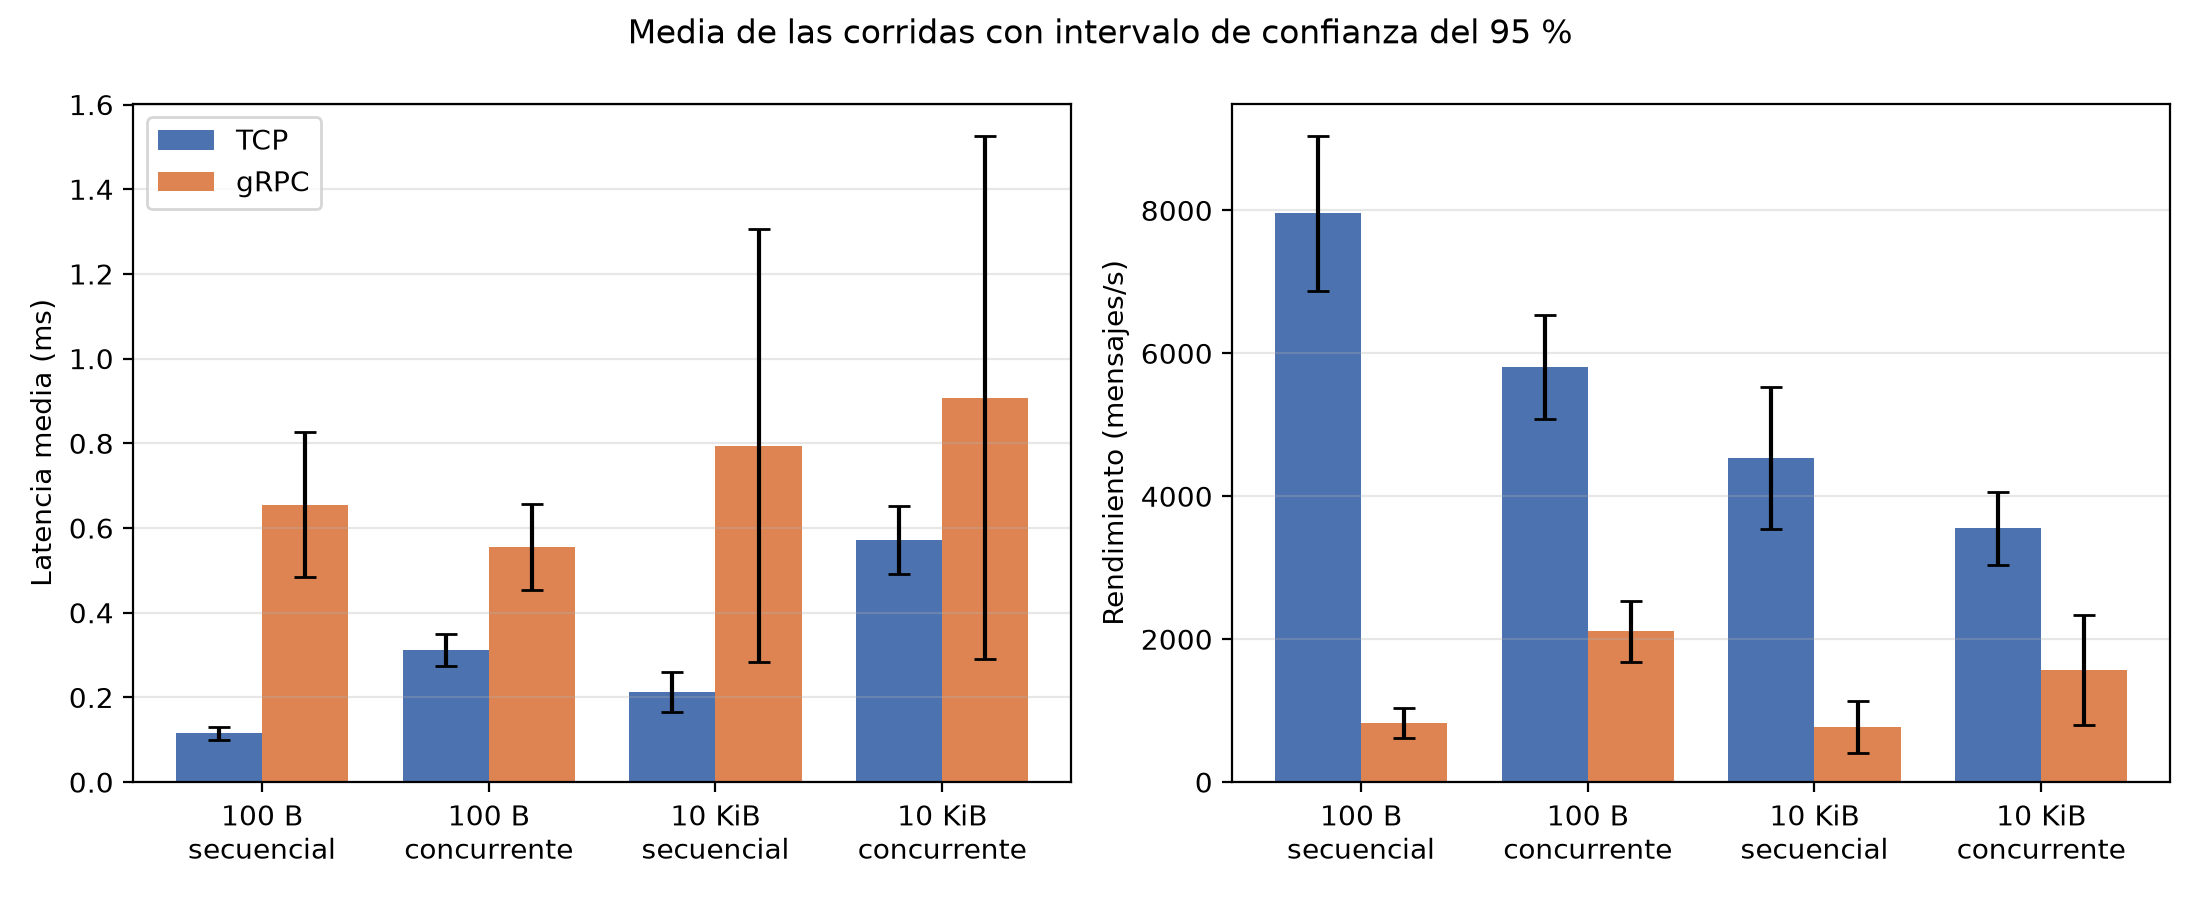
\includegraphics[width=\textwidth]{../analysis/resultados/grafico_barras.png}
\caption{Latencia media y rendimiento con intervalo de confianza del 95~\%}
\label{fig:barras}
\end{figure}
